\section{Experimental Results}
\noindent \textbf{Amplification}\\
As mentioned before, the term "DNS reflection and amplification attack" derives from the two key elements involved in the attack methodology. In particular, to achieve amplification the attacker queries the DNS server, which will reply with larger responses than the original requests. In our project, we conducted various tests to explore different amplification factors based on the DNS request used.\\
We have compiled a summary table showcasing the types of DNS requests used, the corresponding response dimensions, and the amplification factors achieved. The table, shown below, provides a comprehensive overview of these metrics.
\begin{table}[H]
    \centering
    \resizebox{\columnwidth}{!}{%
        \begin{tabular}{|l|c|c|c|c|c|}
            \hline
            \textbf{Type} & \textbf{Request} & \textbf{A} & \textbf{MX} & \textbf{NS} & \textbf{ANY} \\
            \hline
            \textbf{Dimension (bytes)} & 74 & 108 & 306 & 330 & 540 \\
            \hline 
            \begin{tabular}[c]{@{}c@{}}\textbf{Amplification} \\ \textbf{Factor}\end{tabular} & - & 1.46 & 4.14 & 4.46 & 7.30 \\
            \hline 
        \end{tabular}%
    }
    \label{tab:dns-amplification}
\end{table}
\noindent \textbf{Effects on the Target}\\
To assess the effects of the DNS reflection attack, various metrics of the targeted system were measured with regards to performance and network aspects. Regarding the network, the target was used as the primary vantage point, and latency was measured using the ping and dig command tools. The measurement process was divided into three sections to analyze the performance differences. Initially, measurements were taken for a minute without any attack. This established a baseline for normal system performance. Subsequently, a two-minute attack was executed, involving the transmission of 10,000 packets per second to the DNS server by multiple attackers. Finally, an additional minute of measurements without any attack was conducted to detect any potential lingering disturbance effects.\\
The latency graph related to DNS queries presented in Figure \ref{fig:Query_MA_ANY1} visually demonstrates the impact of the attack over time. To improve visualization, a moving average of the latency time was applied, revealing a clear trend of increased latency during the attack. This trick becomes particularly helpful considering the inherent instability of latency measurements.
\begin{figure}[H]
    \centering
    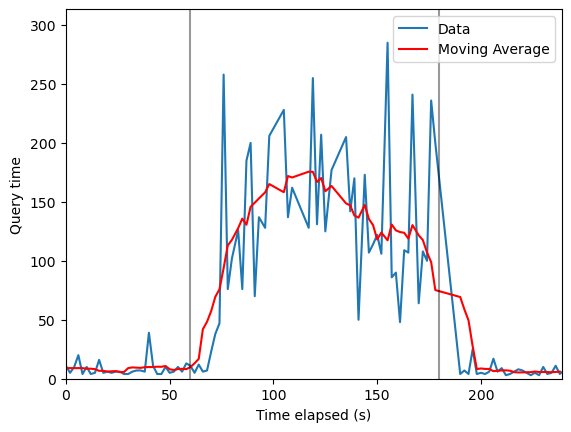
\includegraphics[width=\columnwidth]{Sections/Images/Query_MA_ANY.png}
    \caption{Evolution of the query time over the course of the test with the records of type ANY. The moving average better shows how the latency changes.}
    \label{fig:Query_MA_ANY1}
\end{figure}
\noindent To gain deeper insights into the impact of the DNS reflection attack, it was essential to explore the actual data and analyze the timings of different types of requests. Figure \ref{fig:Boxplots_Query1} showcases the boxplots of query times, illustrating the system under attack with different record types in comparison to the baseline case. \\
\begin{figure}[H]
    \centering
    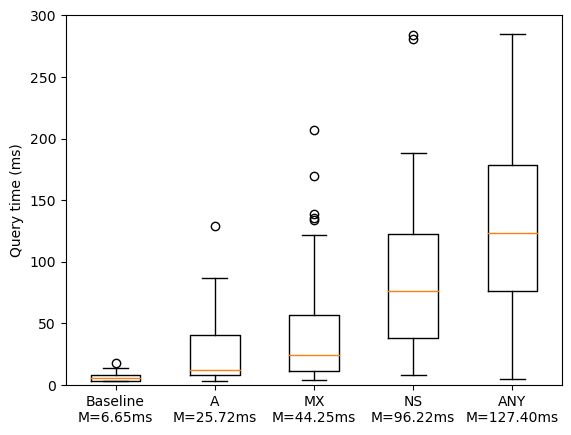
\includegraphics[width=\columnwidth]{Sections/Images/Boxplots_Query.png}
    \caption{Boxplots of the query times with the system under attack with different record types, compared to the baseline case.}
    \label{fig:Boxplots_Query1}
\end{figure}
\noindent By comparing the mean response times during the attack with those observed in the baseline period, we could quantify the magnitude of the latency increase caused by the attack.\\
The results demonstrated that a larger amplification factor corresponds to higher latency. Even in the case of record type A, which typically has a small amplification factor, a noticeable effect on the query time was observed. Remarkably, records of type MX and NS, despite having similar amplification factors (both around 300), exhibited distinct effects on latency. The mean query time for MX records was found to be approximately 44 ms, while NS records had a mean of 96 ms. This discrepancy can be attributed to the resource allocation or in general to the configuration of the DNS server handling the requests.\\
Furthermore, certain cases surpassed the threshold of 100 ms, particularly in the case of the RR ANY record. This indicates that such an attack would have a noticeable impact on the targeted system, for example during web browsing activities. Latencies exceeding this threshold can result in perceptible delays and interruptions, potentially compromising the overall user experience.\\
This analysis provided valuable information on the performance degradation experienced by the targeted system under the influence of the DNS reflection attack.\\
In addition to analyzing the query times using DNS-related tools, we also conducted a similar analysis using the ping command-line tool. The purpose of this analysis was to assess the impact of the DNS reflection attack on overall system latency, beyond just the DNS requests.\\
\begin{figure}[H]
    \centering
    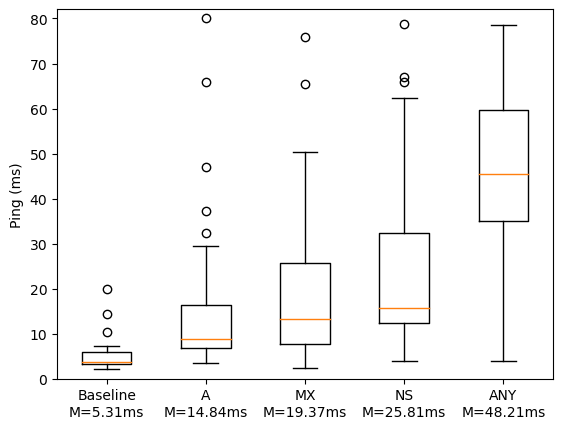
\includegraphics[width=\columnwidth]{Sections/Images/Boxplots_Ping.png}
    \caption{Boxplots of the ping times with the system under attack with different record types, compared to the baseline case.}
    \label{fig:Boxplots_Ping1}
\end{figure}
Surprisingly, as shown in Figure \ref{fig:Boxplots_Ping1} the results obtained from the ping analysis revealed that the latency did not increase significantly during the attack. The highest mean latency observed was approximately 48 ms for the RR of type ANY. \\
This finding suggests that the DNS reflection attack primarily affects the DNS requests themselves, rather than causing widespread disruption to the entire system.\\
During the attacks we also examined the effects of the DNS reflection attack on system resources, specifically RAM and CPU utilization. Our analysis aimed to determine whether the attack had any noticeable impact on these critical resources.\\
Surprisingly, the results revealed that the attack had no significant impact. The resource usage remained within normal ranges, comparable to the baseline measurements taken during the pre-attack phase.\\
\noindent \textbf{Server Performance}\\
Based on the type, victim and server have different performances.\\
%\begin{figure}[H]
%    \centering
%    
\includegraphics[width=\columnwidth]{Sections/Images/example.png}
%   \caption{Example image on one column}
%    \label{fig:example}
%\end{figure}
\noindent Text after the image.\\
